
%%%%%%%%%%%%%%%%%%%%%%%%%%%%%%%%%%%%%%%
%
%	Avi Schwarzschild and Andres Soto
%	APMA 4301: Numerical Methods for PDEs 
% Final Project: Multigrid
%
%%%%%%%%%%%%%%%%%%%%%%%%%%%%%%%%%%%%%%%

\documentclass[pdftex,12pt,a4paper]{article}
\usepackage{amsmath}
\usepackage{amssymb}		% packages that allow mathematical formatting
\usepackage{graphicx}		% package that allows you to include graphics
\usepackage{setspace}		% package that allows you to change spacing
%\onehalfspacing				% text become 1.5 spaced
\usepackage{fullpage}		% package that specifies normal margins
\addtolength{\topmargin}{-.25 in}
\usepackage{fancyhdr}
\usepackage[table]{xcolor}
\usepackage{amsmath}
\usepackage{listings}
\pagestyle{fancy}
\setlength{\headsep}{.5in}
\newcommand{\HRule}{\rule{\linewidth}{0.5mm}}
\graphicspath{ {images/} }
\lstset{basicstyle=\ttfamily}
	
%-- Begin the body below ---%

\begin{document}
\lhead{Multigrid, \today}
\rhead{Schwarzschild and Soto \thepage}

\begin{titlepage}
\begin{center}


% Title


\HRule \\[0.4cm]
{ \huge \bfseries An Exploration of Multigrid Methods \\[0.4cm] }

\HRule \\[1.5cm]

\LARGE Numerical Methods for PDEs 4301\\[0.5cm]


Avi Schwarzschild and Andres Soto \\


\begin{minipage}{0.4\textwidth}
\end{minipage}

\vfill

% Bottom of the page
{\small UNIs: aks2203 and ads2206}


\end{center}
\end{titlepage}
\vspace{2 cm}

\begin{abstract}
    We used both and one and two dimenssional poisson problems to study multigrid methods for solving partial differential equations. Using iterative solvers for linear systems we show how coarsening the descritization can lead to approximations which converge to the true solution of the PDE with fewer iterations of the solver. 
\end{abstract}
%-- Sections correspond to problem numbers --%

\section{Motivation}
   
    \paragraph*{} The motivation for using coarser grids, while convergences analysis shows that finer grids should lead to more accurate approximations, comes from an observation about waves, descritizations, and aliasing. The iterative methods, often referred to as smoothers, smooth out error such that in the earlier iterations it is the high frequency components of the error that vanish first. As the algorithms sweep more times the error gets smoother, containing lower frequencies and tending toward zero. The trouble with the classical iterative methods like this is that low frequencies in the error can take many iterations to smooth. In general these iterative methods are $\mathcal{O}(n^2)$. Thus, some improvement in speed is desired.

    The standard iterative methods for solving elliptic PDEs, often have a propety in which the smoothing rate is not only small but also independent of the grid spacing $h$.  Looking at a numerical example in which we apply weighted Jacobi iteration with $\omega = \frac 2 3$ to the problem $u''(x) = 0$ with zero boundary conditions gives us insight into this phenomena. Our initial guess is a fourier mode that looks like: 

    $$
    w_j = \sin \left( \frac{jk \pi}{N}\right) ~~ 0 \leq j \leq N \text{ and } 1 \leq k \leq N-1$$
    Here $N-1$ is the number of interior points.  A convergence analysis gives us:  

    \begin{figure}[h]
	\centering
	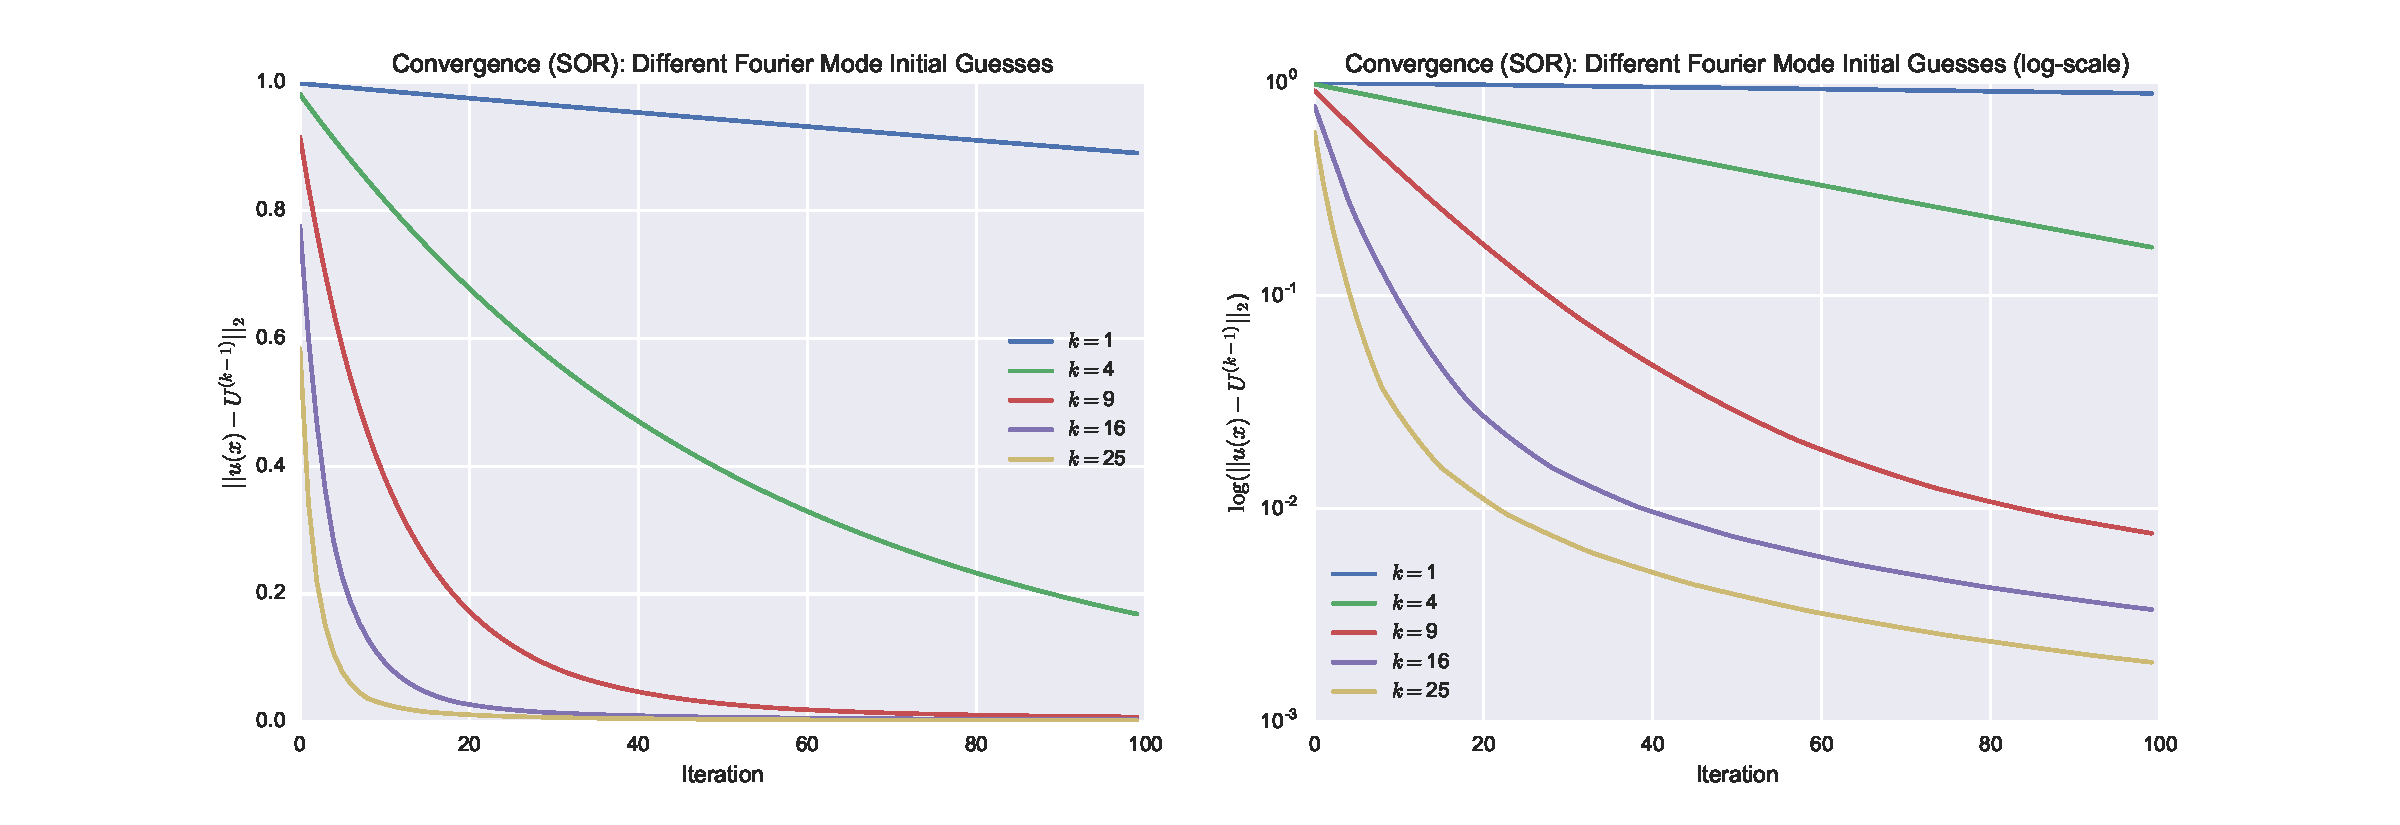
\includegraphics[scale=0.4]{../plots/convergence_sor_diff_modes-motivation.pdf}
	\end{figure}

    We see that error clearly decreases with each relaxation sweep but that the rate of decrease is much more faster for high frequency initial guesses than low frequency ones.  Of course the first way to improve a relaxation is to increase the number of iterations, or improve the initial guess, however, relaxations on a coarser grid is less expensive.  Moreover, smooth components on a fine grid projected onto a coarser grid look more oscillatory.  If we look at fourier modes associated with a mesh of discretization $h$, then we have:
    $$w_{k, 2j}^h = \sin \left( \frac{2jk \pi}{N}\right) =  \sin \left( \frac{jk \pi}{N/2}\right) = w_{k, j}^{2h} ~~ 1 \leq k < \frac N 2 $$.  This seemingly trivial manipulation reeaveals that in passing from a fine grid to coarse grid, the smooth wave becomes more sinusoidal and gains frequency.  

    \paragraph*{} From the Shannon Sampling Theorem we know that to retain all of the wave information, we need the descritization to have just over two points per wavelength.\footnote{C. E. Shannon, ``Communications in the presence of noise'', Proc. IRE, vol. 37, pp. 10-21, Jan. 1949.} The implication of this on our work is that the highest frequency in the error is determined by the mesh grid. Knowing this, we can coarsen the grid so that we have fewer smaple points of the error function and then the low frequencies with be among the higher ones still contained in the coarse-grid error. By smoothing the error on this coarser grid we can eliminate more components of the error than we could without the coarsening. We leave the explanation and implimentation of this for later sections.

\section{ Multigrid Method}

\paragraph{} In this section, we will consider the theory and analyze why multigrid methods work so well.  We will delve deep into gaining some understanding of the linear algebraic implications of mesh restriction and interpolation.  More importantly, we will look at the spectral picture of the multigrid method.  The standard cycle of multigrids is the standard V cycle which looks like: 

\subsection{A Brief Overview}
The basic structure of the multigrid method is that the relaxation scheme underlying each layer possess the smoothing property.  This motivated the coarser grid due to their slow convergence rate.  Multigrid methods further integrate error correction methods by first approximating the residual $r = f - Av$, where $v$ is an approximation and $A$ represents the matrix associated with the iterative method. 

There are two main ideas that come into play in multigrid.  The firstis that coarser grids can be used to improve initial guesses and is the basis of a strategy called nested iteration.  The second idea incorporates utilizing the residual of each smoothing operation at some mesh level in order to correct.  This is the basis of coarse grid correction.  Both of these strategies together lead us to the Full Multigrid Cycle.  

One main question to consider is how integrid transfers work.  Common practice in the multigrid literature for 1d and 2d problems is to interpolate and restrict across different mesh grids.  These linear mappings are of course defined by matrices which are $T_{2h}^h$ and $R_h^{2h}$ (interpolation and restriction, respectively).  Our interpolation matrix in 1d does $T_{2h}^h \mathbf{v}^{2h} = v_j^{2h}$:

$$
v_{2j}^h = v_j^{2h} ~ \text{ and } ~ v_{2j+1}^h = \frac 1 2 ( v_j^{2h} + v_{j+1}^{2h}) ~~  0 \leq j \leq \frac N 2 - 1
$$
In two dimensions this looks like: 

$$
v_{2i, 2j}^h = v_{ij}^{2h} ~~ \text{ and } v_{2i+1, 2j}^h = \frac 1 2 \left( v_{ij}^{2h} + v_{i+1, j}^{2h} \right) \text{ and } v_{2i, 2j+1}^h = \frac 1 2 \left( v_{ij}^{2h} + v_{i, j+1}^{2h} \right)
$$
$$ 
v_{2i+1, 2j+1}^h = \frac 1 4 \left( v_{ij}^h + v_{i+1, j}^{2h} + v_{i, j+1}^{2h} + v_{i+1, j+1}^{2h} \right) ~~ 0 \leq i, j \leq \frac N 2 -1
$$


The restrictive matrix in 1d is defined by $R_h^{2h} \mathbf{v}^h = \mathbf{v}^{2h}$ and looks like:
$$
v_j^{2h} = \frac 1 4 \left( v_{2j-1}^h + 2v_{2j}^h + v_{2j+1}^h \right)
$$
In two dimensions this is: 
\begin{equation}
\begin{aligned}
v_{ij}^{2h} = \frac{1}{16} ( 
v_{2i-1, 2j-1}^h + v_{2i-1, 2j+1}^h  + v_{2i+1, 2j-1}^h  + v_{2i+1, 2j+1}^h  + \\ 2 \left( v_{2i, 2j-1}^h + v_{2i, 2j+1}^h + v_{2i-1,2j}^h + v_{2i+1,2j}^h\right) + 4v_{2i, 2j}^h  ) 
\end{aligned}
\end{equation}

An interesting property is that these matrices are transposes of each other up to a constant. 

    \begin{figure}[h]
    \centering
    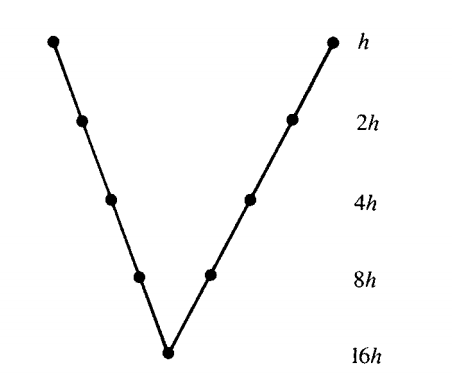
\includegraphics[scale=0.4]{../plots/vcycle.png}
    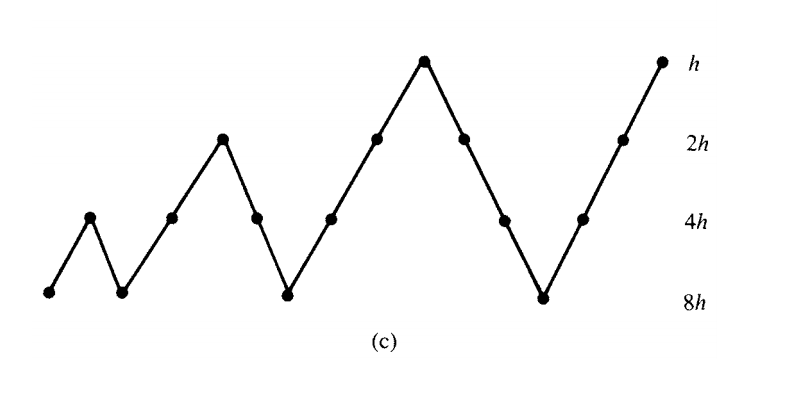
\includegraphics[scale=0.4]{../plots/full-multi-grid-cycle.png}
    \caption{The left figure is a standard Multigrid V Cycle.  The Right figure is a Full Multigrid Cycle (FMV). }
    \end{figure}

With grid transfers well defined, we can discuss a bit more intergrid transfers.  At its core, multigrid methods simply smooth an approximation on some mesh with discretization $h$ and use a coarse grid corrections scheme to understand the error at a coarser mesh to get a better approximation.  This is done iteratively in many fashions.  Below we see two standard cycles of multigrid, both of which we implemented.  


\subsection{The Basic Spectral Picture of Multigrid Methods}
\paragraph{}*Now that we have a better idea of multigrid and their power, we can turn towards understanding some of the mathematical basis behind this powerful method.  We will further develop a spectral picture.  

Transitions from one discretization to another discretization require a mapping of some kind from the current approximation of the true solution or vector to the same vector on the next mesh.  We will adopt the same notation that Briggs introduces. $\Omega^{h}$ represents a grid with spacing $h = \Delta x $, and naturally $\Omega^{2h}$ represents a coarser grid.   $\mathbf{v}^h$ is an approximation of the true solution $\mathbf{u}^h$, and therefore error is $\mathbf{e}^h = \mathbf{u}^h - \mathbf{v}^h$.  The interpolation matrix maps a vector on a coarse mesh, say $\Omega^{2h}$ to $\Omega^{h}$ and is denoted $T_{2h}^h$, while the restriction matrix maps a vector from $\Omega^{h} \rightarrow \Omega^{2h}$ and is denoted by $R_h^{2h}$.  

Assuming, we have $N+1$ total points in our boundary, and $N-1$ interior points, then the restriction matrix $R_h^{2h}$ maps $\mathbb{R}^{N-1} \rightarrow \mathbb{R}^{N/2 -1}$.  Since we have $N-1$ unknown values and are mapping to a lower dimension subspace, then the rank of our restriction matrix is $\frac{N}{2} -1 $ and the null space of the restriction matrix is $\frac{N}{2}$.  Let us explore how this matrix transforms the eigenvalues of our iterative matrix $A^h$ on mesh $\Omega^h$.  The eigenvectors or modes of $A^h$ are given by 
$$\mathbf{w}_{k}^h = \left( \sin\left( \frac{k \pi}{N}\right), \dots, \sin\left( \frac{(N-1)k \pi}{N}\right) \right)$$ where the jth component of the vector is $w_{k,j}^h = \sin\left( \frac{jk \pi}{N}\right)$.  When the restriction operator is applied directly to these vectors we get: 

\begin{equation}
R_h^{2h} \mathbf{w}_k^h = \frac 1 4 \begin{bmatrix}1 & 2 & 1 \\ & 1 & 2 & 1 \\ & & \ddots & \ddots & \ddots \\ & & & 1 & 2 & 1 \end{bmatrix} \mathbf{w}_k^h  
\end{equation}

The jth component of this is:  
\begin{equation}
\Rightarrow \left( R_h^{2h} \mathbf{w}_k^h \right)_j = 
\frac 1 4 \left(\sin\left(\frac{(j-1)k \pi}{N} \right) + 2 \sin\left(\frac{jk \pi}{N} \right)  + \sin\left(\frac{(j+1) k \pi}{N} \right)  \right)
\end{equation}
Using the following two trigonmetric identities, $\sin(\theta_1 + \theta_2) = \sin \theta_1 \cos\theta_2 + \cos\theta_1\sin\theta_2$ and $\cos(2 \theta) = 2 \cos \theta^2 -1$, leads us to: 
$$
\frac 1 4 \left[ 2 \sin\left(\frac{2jk\pi}{N} \right) \cos\left( \frac{k\pi}{N}\right)  + 2 \sin \left( \frac{2jk \pi}{N} \right) \right] =  \sin \left( \frac{jk \pi }{N / 2}\right) \cos^2 \left( \frac{k \pi}{2N} \right) \text{ for } 1 \leq k \leq \frac N 2 $$

What we find is that this result holds for the first $k/2$ eigenvectors or one half of the unknowns.  
\begin{equation}
R_h^{2h} \mathbf{w}_k^h = \cos^2 \left( \frac{k \pi}{2N}\right) \mathbf{w}_k^{2h}, \, \,  1 \leq k \leq \frac N 2 
\end{equation}

The restriction matrix produces a new kth mode of $A^{2h}$ such that the old kth mode of $A^h$ gets multiplied by a constant.  

Applying a similar analysis for when $ \frac N 2 \leq k \leq N -1$, yields

$$
R_h^{2h} \mathbf{w}_{k'}^h = - \sin^2 \left( \frac{k \pi}{2N} \right) \mathbf{w}_k^{2h}, ~~ 1 \leq k \leq \frac N 2 \text{ where } k' = N-ks
$$ 

Essentially, what is going on here is the phenomena of aliasing since the restriction matrix is acting on the $(N-k)$th mode of $A^h$ and multiplying it by a constant multiple of the .  The interpretation behind this result is that the oscillatory modes on $\Omega^h$ cannot be represented in the coarser mesh $\Omega^{2h}$ and the restriction operator transforms these nodes into relatively smooth modes on the coarser mesh.  The reason this matrix has no inverse is because there are two eigenvectors (eigenvector $k$ and eigenvector $N-k$) on $A^h$ that get mapped to the same kth mode on $A^{2h}$.

INCLUDE SOME GRAPHS HERE TO DESCRIBE THIS ALIASING

We define a set $W_k^h$ that takes the span of these complementary nodes (the $(N-k)$th eigenvector and the $k$th eigenvector), $W_k^h = span \{ \mathbf{w}_k^h, \mathbf{w}_{N-k}^h\}$.  We note that: 

$$
w_{N-k, j}^h = \sin \left( \frac{j (N - k) \pi}{N} \right) = \sin\left( j\pi - \frac{jk \pi}{N}\right)
$$

\begin{equation}
\sin(j \pi) \cos \left( \frac{jk \pi}{N} \right) - \cos(j \pi) \sin\left( \frac{jk \pi}{N} \right) =  (-1)^{j+1}\sin\left( \frac{jk \pi}{N} \right) = (-1)^{j+1} w_{k, j}^h
\end{equation}

INCLUDE IMAGE OF COMPLEMENTARY PAIRS

Of course, this two element to one element mapping means that $R_h^{2h}$ contains non-trivial elements in its null space.  Let's take the unit vector $\mathbf{e}_i^h$ on $\Omega^h$, and see how it gets transformed by $R_h^{2h}$.  

\begin{equation}
R_h^{2h} \mathbf{e}_i^h = \begin{bmatrix}1 & 2 & 1 \\ & &  1  & 2 & 1 \\ & & & \ddots &\ddots & \ddots \\ & & & & 1 & 2 & 1 \end{bmatrix} \begin{bmatrix} 0 \\ \vdots \\ 1 \\ \vdots \\ 0 \end{bmatrix}
\end{equation}

We notice that there are two cases due to overlapping ones in the odd columns of $R_h^{2h}$.  If $i$ is odd in $\mathbf{e}_i^h$, then we have a contribution from two rows whereas if $i$ is even, there is only one row contribution from only the component with 2.  We have the following: 

\begin{equation}
R_h^{2h} \mathbf{e}_i^h = 
    \begin{cases}
    \frac 1 4 \left( \mathbf{e}_{ \frac{i-1}{2}}^{2h} + \mathbf{e}_{\frac{i+1}{2}}^{2h} \right) ~~ i \text{ odd }\\

    \frac 1 4 \left( 2 \mathbf{e}_{\frac{i}{2}}^{2h} \right) ~~ i \text{ even }\\
    \end{cases}
\end{equation}

These unit vectors do not form the basis of the null space because this matrix product is not zero.  How about we look at the transformation of these unit vectors under the iterative method first, namely  $R_h^{2h}A^h \mathbf{e}_i^h$.  

\begin{equation}
R_h^{2h}A^h \mathbf{e}_i^h = R_h^{2h} \left( - \mathbf{e}_{i-1}^h + 2 \mathbf{e}_{i}^h - \mathbf{e}_{i+1}^h \right)
\end{equation}

If the $i$ is even then $i-1$ and $i+1$ are odd and we'll get extra terms that do not go to zero, whereas if $i$ is odd, we get: 

\begin{equation}
R_h^{2h}A^h \mathbf{e}_i^h =  -\frac 1 4 \left( 2 \mathbf{e}_{\frac{i-1}{2}}^{2h} \right) + \frac 1 2 \left( \mathbf{e}_{\frac{i-1}{2}}^{2h} + \mathbf{e}_{\frac{i+1}{2}}^{2h} \right) - \frac 1 2 \mathbf{e}_{ \frac{i+1}{2}}^{2h} = 0 
\end{equation}

We see that the vectors $\mathbf{n}_i = A^h \mathbf{e}_i^h$ when $i$ is odd form the basis of the null space of the full weighting operator.  The null space contains both smooth and oscillatory modes of $A^h$ because the vector $A^h \mathbf{e}_i^h$, which is a vector in the range of $A^h$, can be decomposed as a linear combination of the eigenvectors mentioned above.  


Turning our attention to the interpolation matrix, $T_{2h}^h$, which has a reverse mapping from $\mathbb{R}^{N/2 - 1} \rightarrow \mathbb{R}^{N-1}$ and has full rank because there are fewer columns than rows. Like before, we want to ask how this matrix affects the eigenvectors or modes of matrix $A^{2h}$.  Note that this time, we are considering matrix $A^{2h}$ to be consistent with the analysis in restriction.  We know that the jth component of the kth eigenvector of $A^{2h}$ is: 

$$
w_{k,j}^{2h} = \sin \left( \frac{jk \pi}{N /2 } \right) \text{ where } 1 \leq k \leq \frac N 2 \text{ and } 0 \leq j \leq \frac N 2
$$
The jth component of $T_{2h}^h \mathbf{w}_{k}^{2h}$ looks like: 

$$ 
T_{2h}^h \mathbf{w}_k^{2h} = \frac 1 2 \begin{bmatrix} 1 \\ 2 \\ 1 & 1 \\ & 2 \\ & 1 & 1 \\ & & \ddots & \ddots  \end{bmatrix} \mathbf{w}_k^{2h}
$$

$$
( T_{2h}^h \mathbf{w}_k^{2h} )_j = 
\begin{cases}
 \sin\left( \frac{ k(j / 2) \pi }{N/2} \right) ~~ j \text{ even}\\
\frac 1 2 \sin \left( \frac{k \frac{j-1}{2} \pi}{N/2} \right) + \frac 1 2 \sin \left( \frac{k \frac{j+1}{2}\pi}{N/2} \right) ~~ j \text{ odd}
\end{cases}
$$

For j odd we have: 
$$
( T_{2h}^h \mathbf{w}_k^{2h} )_j = \frac 1 2 \sin \left( \frac{k (j-1) \pi}{N} \right) + \frac 1 2 \sin \left( \frac{k (j+1)\pi}{N} \right)
$$

Using the trigonemtric sum identity and double angle cosine identity $2 \cos^2 \theta -1 = \cos 2 \theta $, we get that for the $j$ is odd case: 

$$ \Rightarrow
\sin \left( \frac{kj \pi}{N}\right) \cos \left( \frac{k \pi}{N}\right) = \sin \left( \frac{kj \pi}{N}\right)  \left(2 \cos^2 \left( \frac{k \pi}{2N} \right)  - 1  \right) 
$$
$$ \Rightarrow
\sin \left( \frac{kj \pi}{N}\right) \cos^2 \left( \frac{k \pi}{2N} \right) + \sin \left( \frac{kj \pi}{N}\right) \left( \cos^2 \left( \frac{k \pi}{2N} \right) - 1\right) \text{ and we have } k = N - k'$$ 

$$ \Rightarrow 
\sin \left( \frac{kj \pi}{N}\right) \cos^2 \left( \frac{k \pi}{2N} \right) - \sin \left( \frac{(N-k')j \pi}{N}\right) \sin^2 \left( \frac{k \pi}{2N} \right)
$$

$$ \Rightarrow
\sin \left( \frac{kj \pi}{N}\right) \cos^2 \left( \frac{k \pi}{2N} \right)  - \sin^2 \left( \frac{k \pi}{2N} \right) \left[ \sin(j \pi) \cos \left( \frac{k' j \pi}{N}\right) - \cos( j \pi) \sin \left( \frac{k' j \pi}{N}\right)\right]
$$

$$\Rightarrow
\sin \left( \frac{kj \pi}{N}\right) \cos^2 \left( \frac{k \pi}{2N} \right)  -\sin^2 \left( \frac{k \pi}{2N} \right)  \left[ (-1)^{j+1} \sin \left( \frac{k' j \pi}{N}\right) \right] \text{ and because j is odd ... }
$$

\begin{equation}
\cos^2 \left( \frac{k \pi}{2N} \right) \sin \left( \frac{kj \pi}{N}\right)  -\sin^2 \left( \frac{k \pi}{2N} \right) \sin \left( \frac{k' j \pi}{N}\right)
\end{equation}

For the even case, we can do the following: 

$$
( T_{2h}^h \mathbf{w}_k^{2h} )_j = \sin\left( \frac{ k j \pi }{N} \right) = \cos^2 \left( \frac{k \pi}{2N} \right) \sin\left( \frac{ k j \pi }{N} \right) + \sin^2 \left( \frac{k \pi}{2N} \right) \sin\left( \frac{ k j \pi }{N} \right)
$$

In the previous page we showed that complementary nodes are related by just a sign.  Using this we can turn the above expression to take on a similar form. Just like Briggs, we'll define $c_k = \cos^2 \left( \frac{k \pi}{2N} \right)$ and $s_k = \sin^2 \left( \frac{k \pi}{2N} \right)$.  Therefore, for both the even and odd case we can express the new eigenvectors as:  

\begin{equation}
[T_{2h}^h \mathbf{w}_k^{2h}]_j =  \cos^2 \left( \frac{k \pi}{2N} \right) \sin\left( \frac{ k j \pi }{N} \right) - \sin^2 \left( \frac{k \pi}{2N} \right) \sin\left( \frac{ k j \pi }{N} \right) 
\Rightarrow 
 T_{2h}^h \mathbf{w}_k^{2h} = c_k \mathbf{w}_k^h - s_k \mathbf{w}_k^h
\end{equation}

The takeaway of all this tedious, trigonemtric algebra is that the interpolation matrix in some way excistes the kth mode in $\Omega^{2h}$ to produce two modes on the finer mesh $\Omega^h$.  

A basis for the range of interpolation is of course given by the columns of $T_{2h}^h$ because it is full rank (all of its columns are linearly independent).  Just like the null space of the restriction matrix, these basis vectors can be decomposed as a linear combination of the modes of $A^h$ and hence reveal that the column space of the interpolation matrix contains both smooth and oscillatory nodes of $A^h$ (see Briggs).  

The purpose of all this analysis on these two matrices subspaces and their affect on the modes of $A^h$ is because the crux of multigrid methods is the \textit{coarse grid correction scheme}.  This scheme is a residual correction scheme that maps the residual of n iterative method on some mesh $\Omega^h$ to a coarser mesh to solve for error.  This error is then interpolated upwards to obtain a better approximation.  Essentially, coarse grid correction (CGC) is a series of matrix products.  
\begin{enumerate}
\item We start with an approximation, $\mathbf{v}^h$ to our true solution, $\mathbf{u}^h$ and relax $\nu$ times. $\mathbf{v}^h \leftarrow P^{ \nu} \mathbf{v}^h $, where $P$ is a relaxation scheme

\item Obtain a residual $\mathbf{r}^h$ and restrict it: $ \mathbf{r}^{2h}  = R_h^{2h} ( \mathbf{f}^h -  A^h \mathbf{v}^h )$

\item Solve the residual equation: $\mathbf{v}^{2h} = (A^{2h})^{-1} \mathbf{f}^{2h} $

\item Correct the approximation on the original mesh $\Omega^h$: $\mathbf{v}^h \leftarrow \mathbf{v}^h + T_{2h}^h \mathbf{v}^{2h} $
\end{enumerate}

These 4 steps can be summarized as a series of matrix products: 

\begin{equation}
\mathbf{v}^h \leftarrow P^{\nu} \mathbf{v}^h + T_{2h}^h (A^{2h})^{-1} R_h^{2h} ( \mathbf{f}^h -  A^h P^{\nu} \mathbf{v}^h )
\end{equation}
Naturally, this must statisfy: 

\begin{equation}
\mathbf{u}^h = P^{\nu} \mathbf{u}^h + T_{2h}^h (A^{2h})^{-1} R_h^{2h} ( \mathbf{f}^h -  A^h P^{\nu} \mathbf{u}^h )
\end{equation}
Taking their difference and considering this difference as the coarse grid correction operator (as Brigsgs does, page 74), we get a matrix operator: 

\begin{equation}
\left[ I - T_{2h}^h (A^{2h})^{-1} R_h^{2h} A^h \right] P^{\nu}
\end{equation}

Considering this whole series of products and sums as one operation, Briggs states that in the scenario in which we do not relax, $\nu = 0$, then the subspaces $W_k^h = \text{span} \{w_k^h, w_{k'}^h \}$ is an invariant subspace.  


We will endeavour to prove this.  Without any relaxation, our operator is: 

$$
I - T_{2h}^h (A^{2h})^{-1} R_h^{2h} A^h
$$
In a homework problem, we found that kth eigenvalue of the matrix $A^h$ is $\lambda_k^h = 4 \sin^2 \left( \frac{k \pi}{2N} \right)$.  We therefore have: 

\begin{enumerate} 
\item $ A^h \mathbf{w}_k^h = \lambda_k^h \mathbf{w}_k^h$
\item $ R_j^{2h}A^h \mathbf{w}_k^h  = \lambda_k^h \cos^2 \left( \frac{k \pi}{2N}\right) \mathbf{w}_k^h $
\item $ (A^{2h} )^{-1} R_j^{2h}A^h \mathbf{w}_k^h = \lambda_k^h \cos^2 \left( \frac{k \pi}{2N}\right) (A^{2h})^{-1} \mathbf{w}_k^{2h} = \frac{\lambda_k^h}{\lambda_k^{2h}} \cos^2\left( \frac{k \pi}{2N}\right)\mathbf{w}_k^{2h}$

\item $T_{2h}^h(A^{2h} )^{-1} R_j^{2h}A^h \mathbf{w}_k^h =  \frac{\lambda_k^h}{\lambda_k^{2h}} \cos^2\left( \frac{k \pi}{2N}\right) T_{2h}^h \mathbf{w}_k^{2h} =
\frac{\lambda_k^h}{\lambda_k^{2h}} \cos^2\left( \frac{k \pi}{2N}\right) \left[ c_k \mathbf{w}_k^h - s_k \mathbf{w}_{k'}^h \right]$
\item Our final expression for the change on $\mathbf{w}_k^h$ by this coarse grid correction operator is: 

$$
\mathbf{w}_k^h - \frac{\lambda_k^h}{\lambda_k^{2h}} \cos^2\left( \frac{k \pi}{2N}\right) \left[ c_k \mathbf{w}_k^h - s_k \mathbf{w}_{k'}^h \right]
$$ 

\end{enumerate}

Plugging in our eigenvalues into this, we obtain: 

\begin{equation}
\mathbf{w}_k^h  - \frac{4 \sin^2 \left( \frac{k \pi}{2N} \right)}{4 \sin^2 \left( \frac{k \pi}{N} \right)} \cos^2\left( \frac{k \pi}{2N}\right) \left[ c_k \mathbf{w}_k^h - s_k \mathbf{w}_{k'}^h \right]
\end{equation}

\begin{equation}
\left(1 - \frac{ \sin^2 \left( \frac{k \pi}{2N} \right) \cos^4\left( \frac{k \pi}{2N}\right) }{ \sin^2 \left( \frac{k \pi}{N} \right)}  \right)\mathbf{w}_k^h  + \frac{ \sin^4 \left( \frac{k \pi}{2N} \right) \cos^2\left( \frac{k \pi}{2N}\right) }{ \sin^2 \left( \frac{k \pi}{N} \right) }  \mathbf{w}_{k'}^h
\end{equation}

Using the double angle formula  $\sin 2 \theta = 2\sin \theta \cos \theta $ and $\cos^2 \theta + \sin^2 \theta = 1$, we can show (a lot of algebra): 

$$
\left( 1 -  \frac{\cos^2 \left( \frac{k \pi}{2N}\right)}{4} \right) \mathbf{w}_k^h + \frac 1 4 \sin^2 \left( \frac{k \pi}{2N} \right) \mathbf{w}_{k'}^h
$$

$$\Rightarrow
\left( \frac 3 4 + \frac 1 4 \sin^2\left( \frac{k \pi}{2N}\right) \right) \mathbf{w}_k^h + \frac 1 4 \sin^2 \left( \frac{k \pi}{2N}\right) \mathbf{w}_{k'}^h
$$

If we continue and expand things out, we can show this equals to, $s_k \mathbf{w}_k + s_k w_{k'}$ and hence we obtain invariance of the elemtn $\mathbf{w}_k$.  We need to do this for the element $\mathbf{w}_{k'}$.  To avoid the same type of analysis, we'll rely on Briggs to assert that we get $c_k \mathbf{w}_k + c_k \mathbf{w}_{k'}$.  What this means is that we get smooth and oscillatory results when this coarse grid correction scheme is applied to these complementary modes.  

The power of this method comes from the spectral properties of iterative solvers.  When we introduce $\nu$ steps of relaxation of some iterative method, like Gauss-Seidel or SOR, then we get that our new operator becomes:

\begin{equation}
\left( I - T_{2h}^h (A^{2h})^{-1} R_h^{2h} A^h \right) P^{\nu}
\end{equation}

Note, 
Following the same 5 steps above, we get that (letting $\lambda_k$ be the eigenvalue of P associated with the kth eigenvector $\mathbf{w}_k$)

$$
\left(I - T_{2h}^h (A^{2h})^{-1} R_h^{2h} A^h \right) P^{\nu} \mathbf{w}_k^h = \left(I - T_{2h}^h (A^{2h})^{-1} R_h^{2h} A^h \right) \lambda^{\nu}_k  \mathbf{w}_k^h
$$

What is new this time is a constant term - the eigenvalue! So we get similar results!  The coarse grid correction scheme when operating on $\mathbf{w}_k$ and $\mathbf{w}_{k'}$ returns:

$$
\lambda_k^{\nu} s_k \mathbf{w}_k + \lambda_k^{\nu} s_k \mathbf{w}_{k'} \text{ and } \lambda_k^{\nu}c_k \mathbf{w}_k
+ \lambda_k^{\nu} c_k \mathbf{w}_{k'} ~~~ \text{where } 1 \leq k \leq \frac N 2, ~~ k' = N-k
$$

The smoothing is the dominant term here! It is what makes the oscillatory modes small, while at the same time eliminating smooth modes, reflected in the $s_k$ terms. When all terms are small particularyly for small modes $k$ relative to $N/2$ or when the number of relaxation increases, the end result is a complete process where both types of eigenvectors (low frequency and high frequency modes) are well damped. This is the spectral picture of the multigrid method








\section{One Dimensional Problem}
    
    \paragraph*{} For the one dimenssional problem we chose to demonstrate the Poisson problem with Dirichlet boundary conditions as follows:
    
    \begin{equation}
    \begin{aligned}
        \frac{d^2u}{dx^2} &= f(x) ~ , ~~ x \in (a, b), \\
        u(a) &= \alpha, \\
        u(b) &= \beta.
    \end{aligned}
    \end{equation}
    
    The values of $f(x)$, $a$, $b$, $\alpha$, and $\beta$ are specified below for the test example. \\
    \begin{itemize}
        \item Example \#1: 
            \begin{equation*}
                f(x) = -\sin(x) ~ , ~~ a = 0 ~ , ~~ b = 2 \pi ~ , ~~ \alpha = \beta = 0
            \end{equation*}

    \end{itemize}
    The results of our method are presented in the Results section, however we will describe the implementation in the next section first. The analytic solution to this ODE is not a difficult one to derive, and we will not show the derivation here, but we state that the solution is: $$ u(x) = \sin(x) $$

    \subsection{Implementation}   

        \paragraph*{} Regarding implementation, choosing an appropriate data structure is essential to achieving a high level efficency otherwise, the benefits of the multigrid method is lost.  Briggs, in \textit{A Multigrid Tutorial}, adopts arrays as his primary data structure for one-dimensional problems.  We adopted the same strategy and in general, any arbitrary grid will contain $2^{n}-1$ interior grid points plus two boundary points for a total of $2^{n}+1$.  The size of the arrays are transformed across different mesh grids. 

        \paragraph*{} In a dedicated python class, we hold onto several attributes of the problem. The constructor for the one dimenssional problem, takes as input: The descrete domain $x$ (a Numpy array), solution array $u$ whose input serves as the initial guess, boundary endpoints, and the non-homogeneous term $f$ as a function. Holding onto these variable we can then call \lstinline{iterate(), v_sched(), or fmg()} to approximate the solution.

        \paragraph*{\lstinline{iterate()}}calls the iterative solver. The numerical method empolyed is either Gauss-Seidel or Successive Over Relaxation. The pseudocode as well as mathematical analysis of these methods was explained in previous assignments for this course, so we chose to leave that out of this paper. 

        \paragraph*{\lstinline{v_sched()}} intiates a Multi Grid V-Cycle which solves a system $Au = f$ with a coarse grid correction scheme. The pseudocode for the recursive implementation used is as follows:
        \begin{verbatim}
             1 v_sched(u, A, rhs, dx, level):
             2     if this is the coarsest grid:
             3         solve exactly Au = rhs
             4     else:
             5         iterate(u) twice
             6         residue = Au - rhs
             7         coarsen(A, residue)
             8         e = v_sched(0, coarse A, coarse residue, 2*dx, level-1)
             9         interpolate(e) and update u by added the refined e
            10         iterate(new u) twice                
            11     return u

        \end{verbatim}
        The recursive call to \lstinline{v_sched()} is solving a new linear system on the coarser grid. This coarsening is moves through the levels until the problem at hand is small enough to be solved exaclty, in our case using Numpy's linear solver. For the iterative methods called before and after the coarse grid correction,  either Gauss-Seidel or SOR could be chosen, and the number of times of pre and post smoothing are a parameter that can be set.

        \paragraph*{\lstinline{fmg()}} intiates a Full Multi Grid Cycle which solves a system $Au = f$ with a coarse grid correction scheme. The pseudocode for the recursive implementation used is as follows:
        \begin{verbatim}
        1 fmg(u, A, rhs, dx, level):
        2     if this is the coarsest grid:
        3         solve exactly Au = rhs
        4     else:
        5         coarsen(A, u, rhs)
        6         u' = fmg(coarse u, coarse A, coarse rhs, 2*dx, level-1)
        7         u_new = interpolate(u')
        8         u = v_sched(u_new, A, rhs, dx, level)
        9     return u

        \end{verbatim}
        The recursive call to \lstinline{fmg()} is solving a coarser version of the same linear system, $Au = f$. At the coarses level it solves this exaclty and then interoplates the solution back up to the finer grid. After each coarsening/refining stage the fucntion calls \lstinline{v_sched()} solving the finer problem using the coarse grid correction scheme outlined above in pseudocode. 

        \paragraph*{} It is important to note here that the pseudocode would look identical for the two dimenssional problem, becasue the differences are in the details. For two dimensions, there is a fair amount of reshaping vectors and matrices, and the coarsening and interpolating matrices are also slightly different, but because these are only outlined in previous sections and not highlited in the pseudocode, we will not rewrite any pseudocode for the two dimensional problem. 

    \subsection{Results}

        \paragraph*{} From Example \#1 we have solution plots and an error comparison from four runs. Each took the same initialization parameters, other than the choice of iterative solver. (a) GS was computed using only the Gauss-Seidel iteration method; (b) SOR was only using the SOR method; (c) MG was a coarse grid correction cycle method using \lstinline{v_sched()}, above; and (d) FMG was using the Full Multi Grid Cycle outlined above in \lstinline{fmg()}. Below are the solutions and error plots:

        \begin{figure}[h]
            \centering
            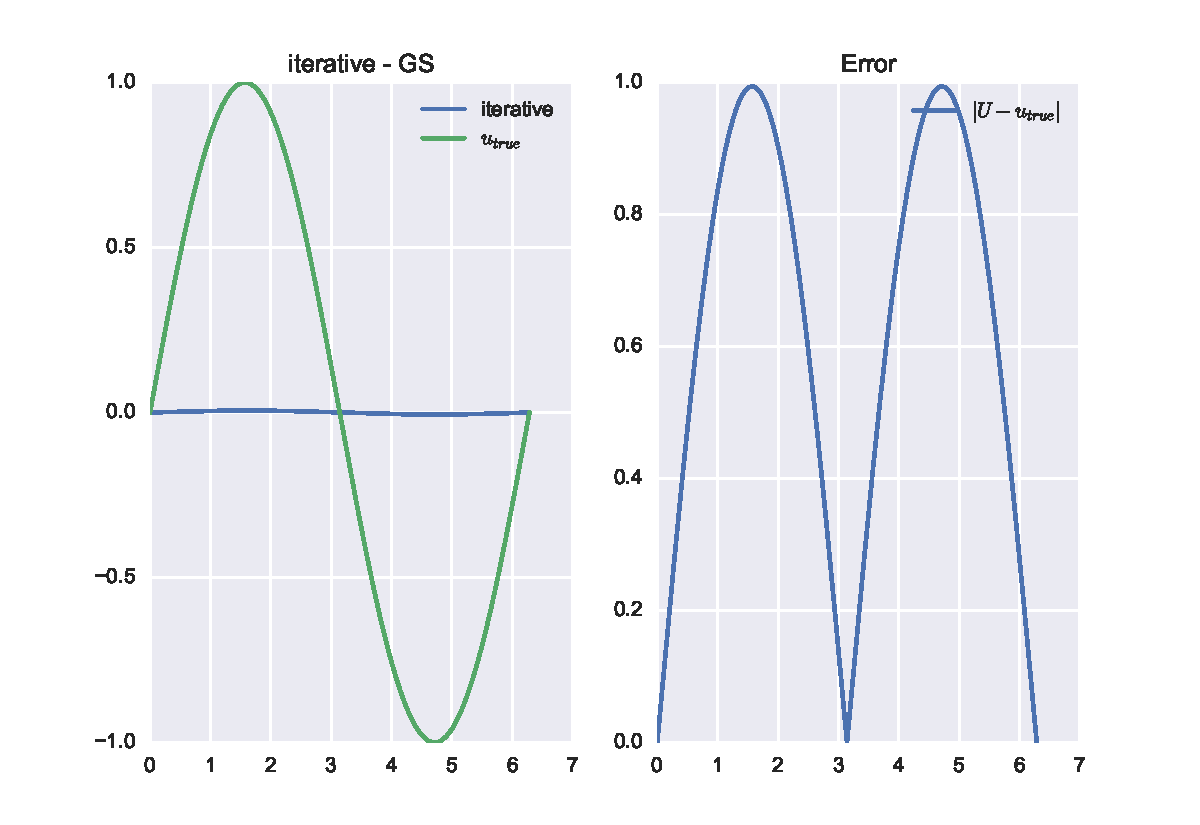
\includegraphics[scale=.4]{../plots/gs_sol_1d.pdf}
            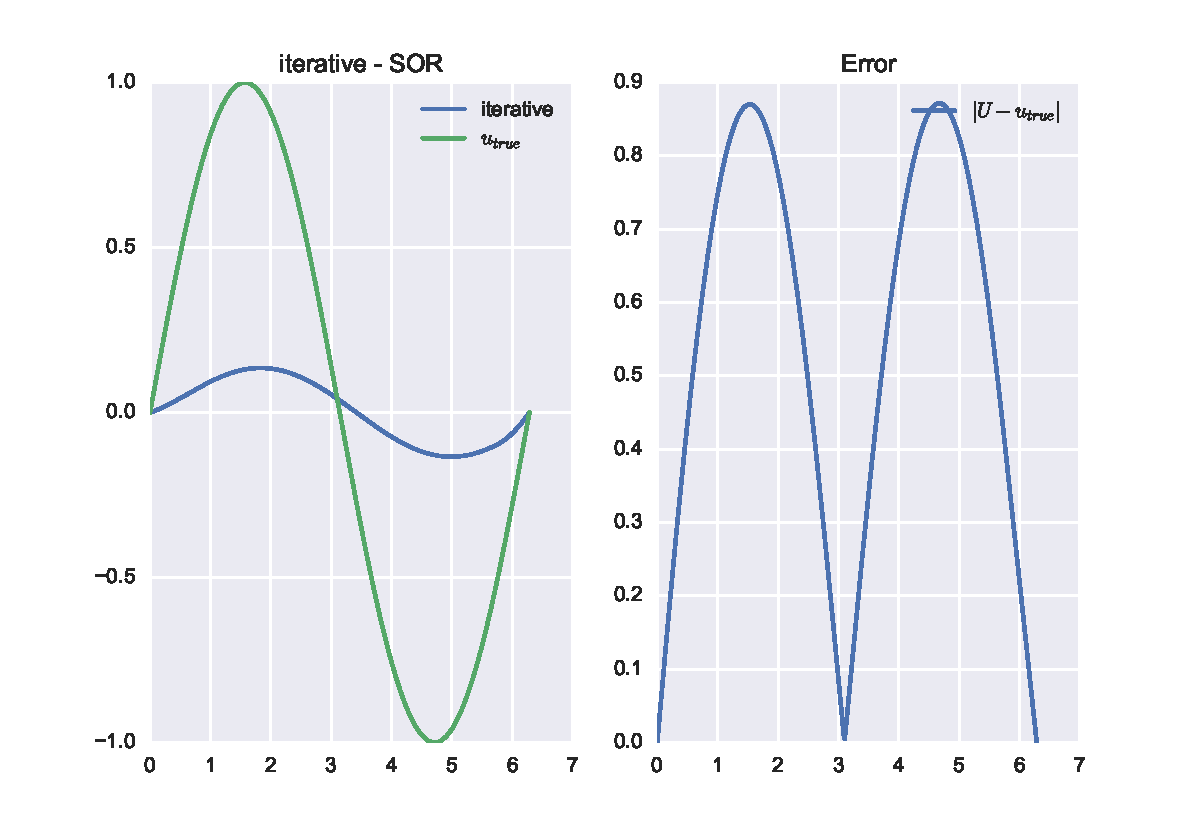
\includegraphics[scale=.4]{../plots/sor_sol_1d.pdf} 
            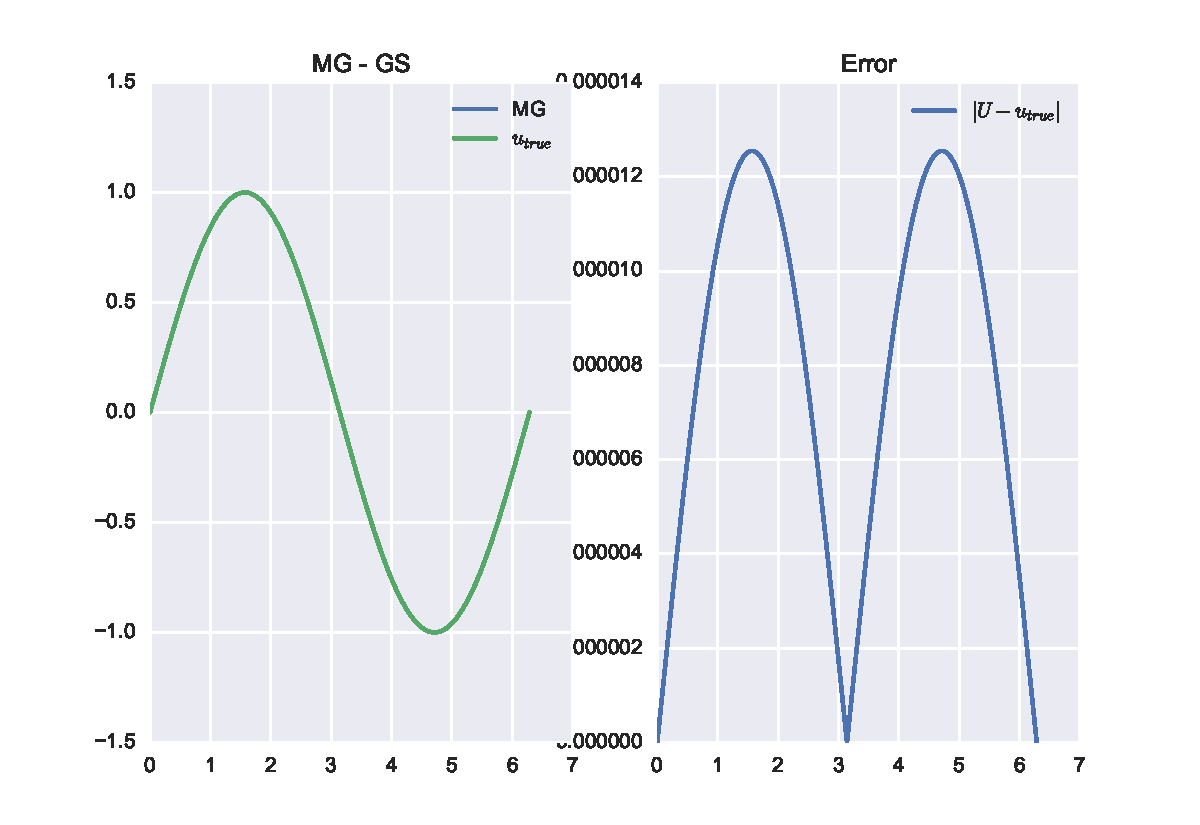
\includegraphics[scale=.4]{../plots/v_sol_1d.pdf}
            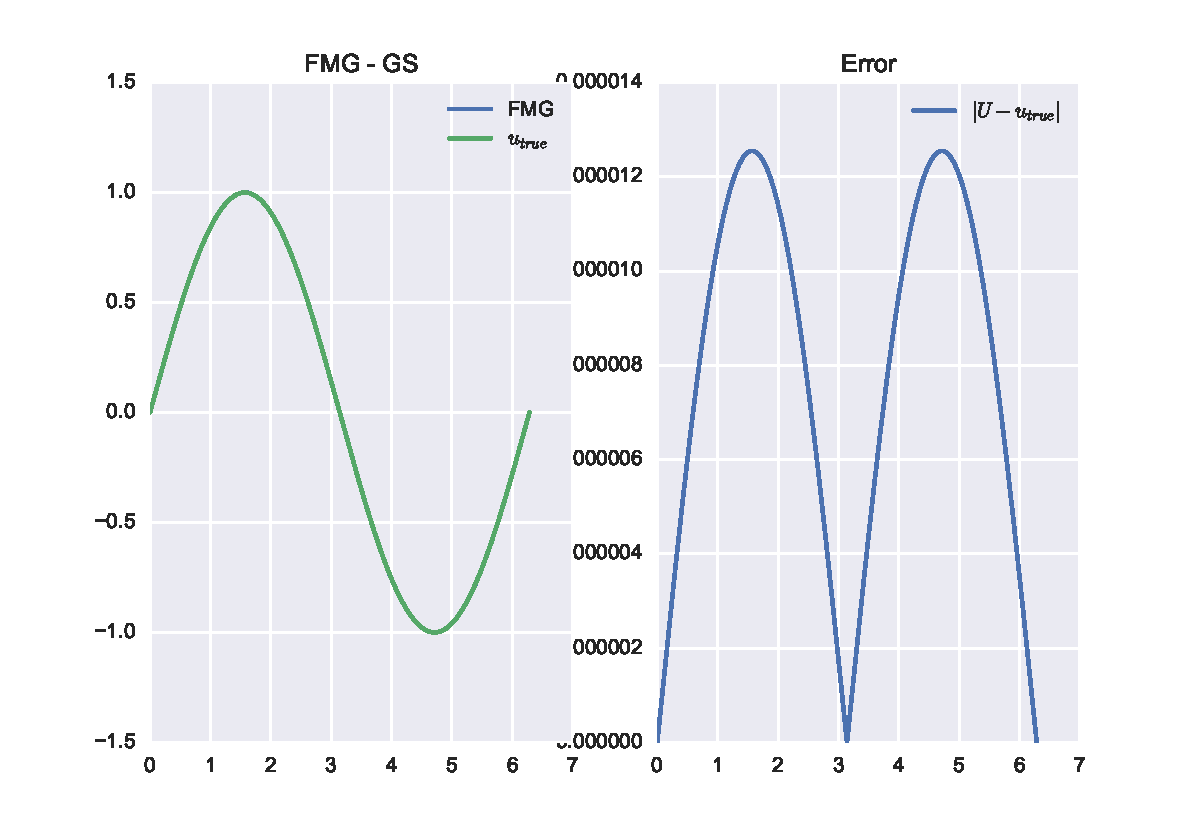
\includegraphics[scale=.4]{../plots/fmg_sol_1d.pdf}
            \caption{top left (a), top right (b), bottom left (c), bottom right (d)}
        \end{figure}

        The error on each plot is interesting, specifically notice the order on the y-axis. Here is the error from each run as a function of effective iteration\footnote{Effective iteration counts the exact number of iteratations when only solving with iterative solvers, but only counts the sweeps on the finest grid when using multigrid.This is justified because by comparison the sweeps on the coarse grids are cheap.} We notice in the bottom plot how much faster the multigrid methods are than the regular iterative solvers. Additionally the error plot explains why in the above plots MG and FMG look so similar -- they have both reached the plateaus in their error. It is not that one method is more accurate in absolute terms, but rather that they converge in many fewer sweeps of the iterative solver.
        \begin{figure}[h]
            \centering
            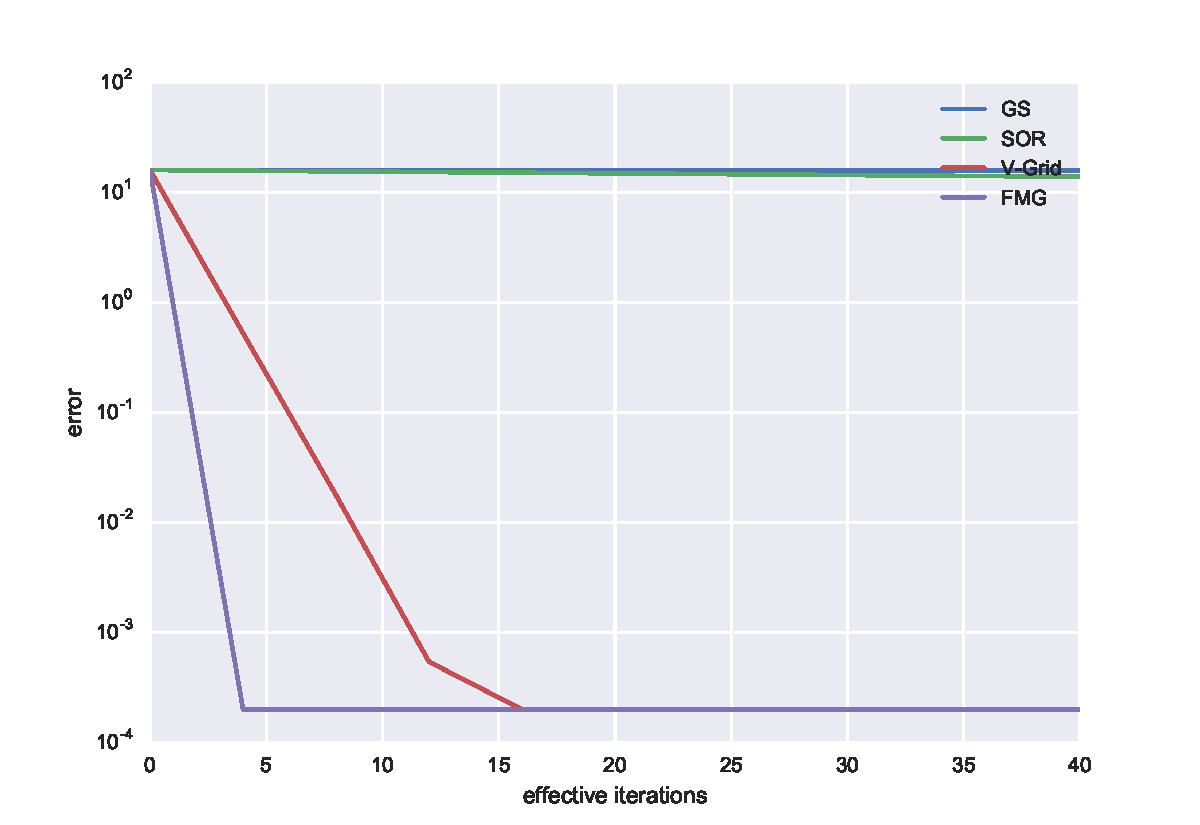
\includegraphics[scale=.75]{../plots/error_1d.pdf}
        \end{figure}      


\section{Two Dimensional Problem}
    \paragraph*{} For the two dimenssional problem we chose to demonstrate the Poisson problem with Dirichlet boundary conditions as follows:
    
    \begin{equation}
    \begin{aligned}
        u_{xx} + u_{yy} &= f(x, y) ~ , ~~ (x, y) \in \Omega, \\
        u|_{\partial \Omega} &= g(x, y), \\
    \end{aligned}
    \end{equation}
    
    The values of $f(x, y)$, $\Omega$, and $g(x, y)$ are specified below for the test example. \\
    \begin{itemize}
        \item Example \#2: 
            \begin{equation*}
            \begin{aligned}
                f(x, y) =& -\frac12\sin(x)\sin(y) ~, ~~ g(x, y) = 0 \\
                \Omega &= [0, 2\pi] \times [0, 2\pi]
            \end{aligned}
            \end{equation*}

    \end{itemize}
    The results of our method are presented in the Results section, however we will describe the implementation in the next section first. The analytic solution to this ODE is not a difficult one to derive, and we will not show the derivation here, but we state that the solution is: $$ u(x) = \sin(x) $$

    \subsection{Results}
        \paragraph*{} From Example \#2 we have solution plots and an error comparison from four runs, jsut like before: (a) GS was computed using only the Gauss-Seidel iteration method; (b) SOR was only using the SOR method; (c) V-Grid was a coarse grid correction cycle method using \lstinline{v_sched()}, above; and (d) FMG was using the Full Multi Grid Cycle outlined above in \lstinline{fmg()}. Below are the solutions and error plots:
        \subsubsection*{}
        
            \begin{figure}[!h]
                \centering
                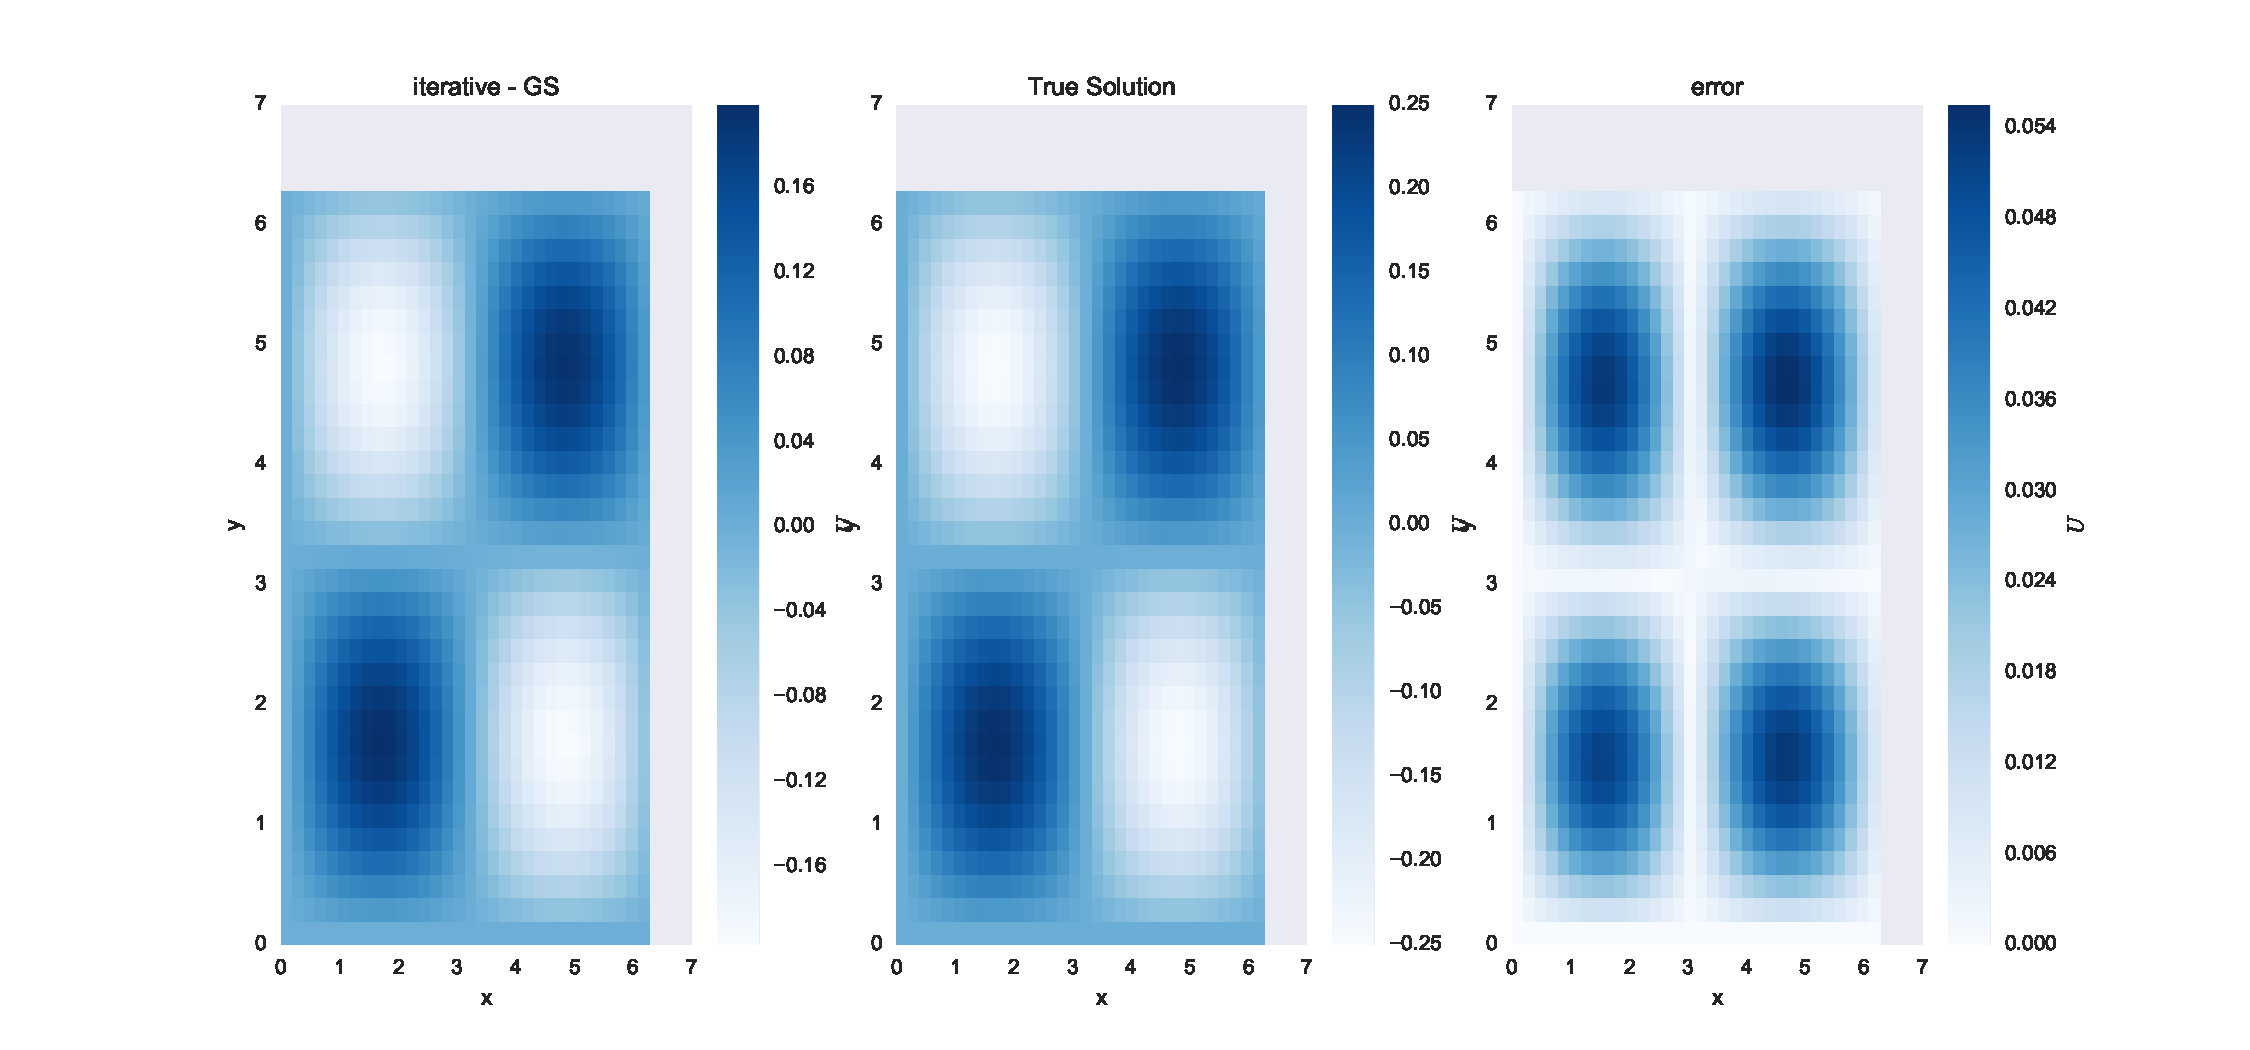
\includegraphics[scale=.5]{../plots/gs_sol_2d.pdf} \\
                \caption{(a)}
            \end{figure}
            
            \begin{figure}[!h]
                \centering
                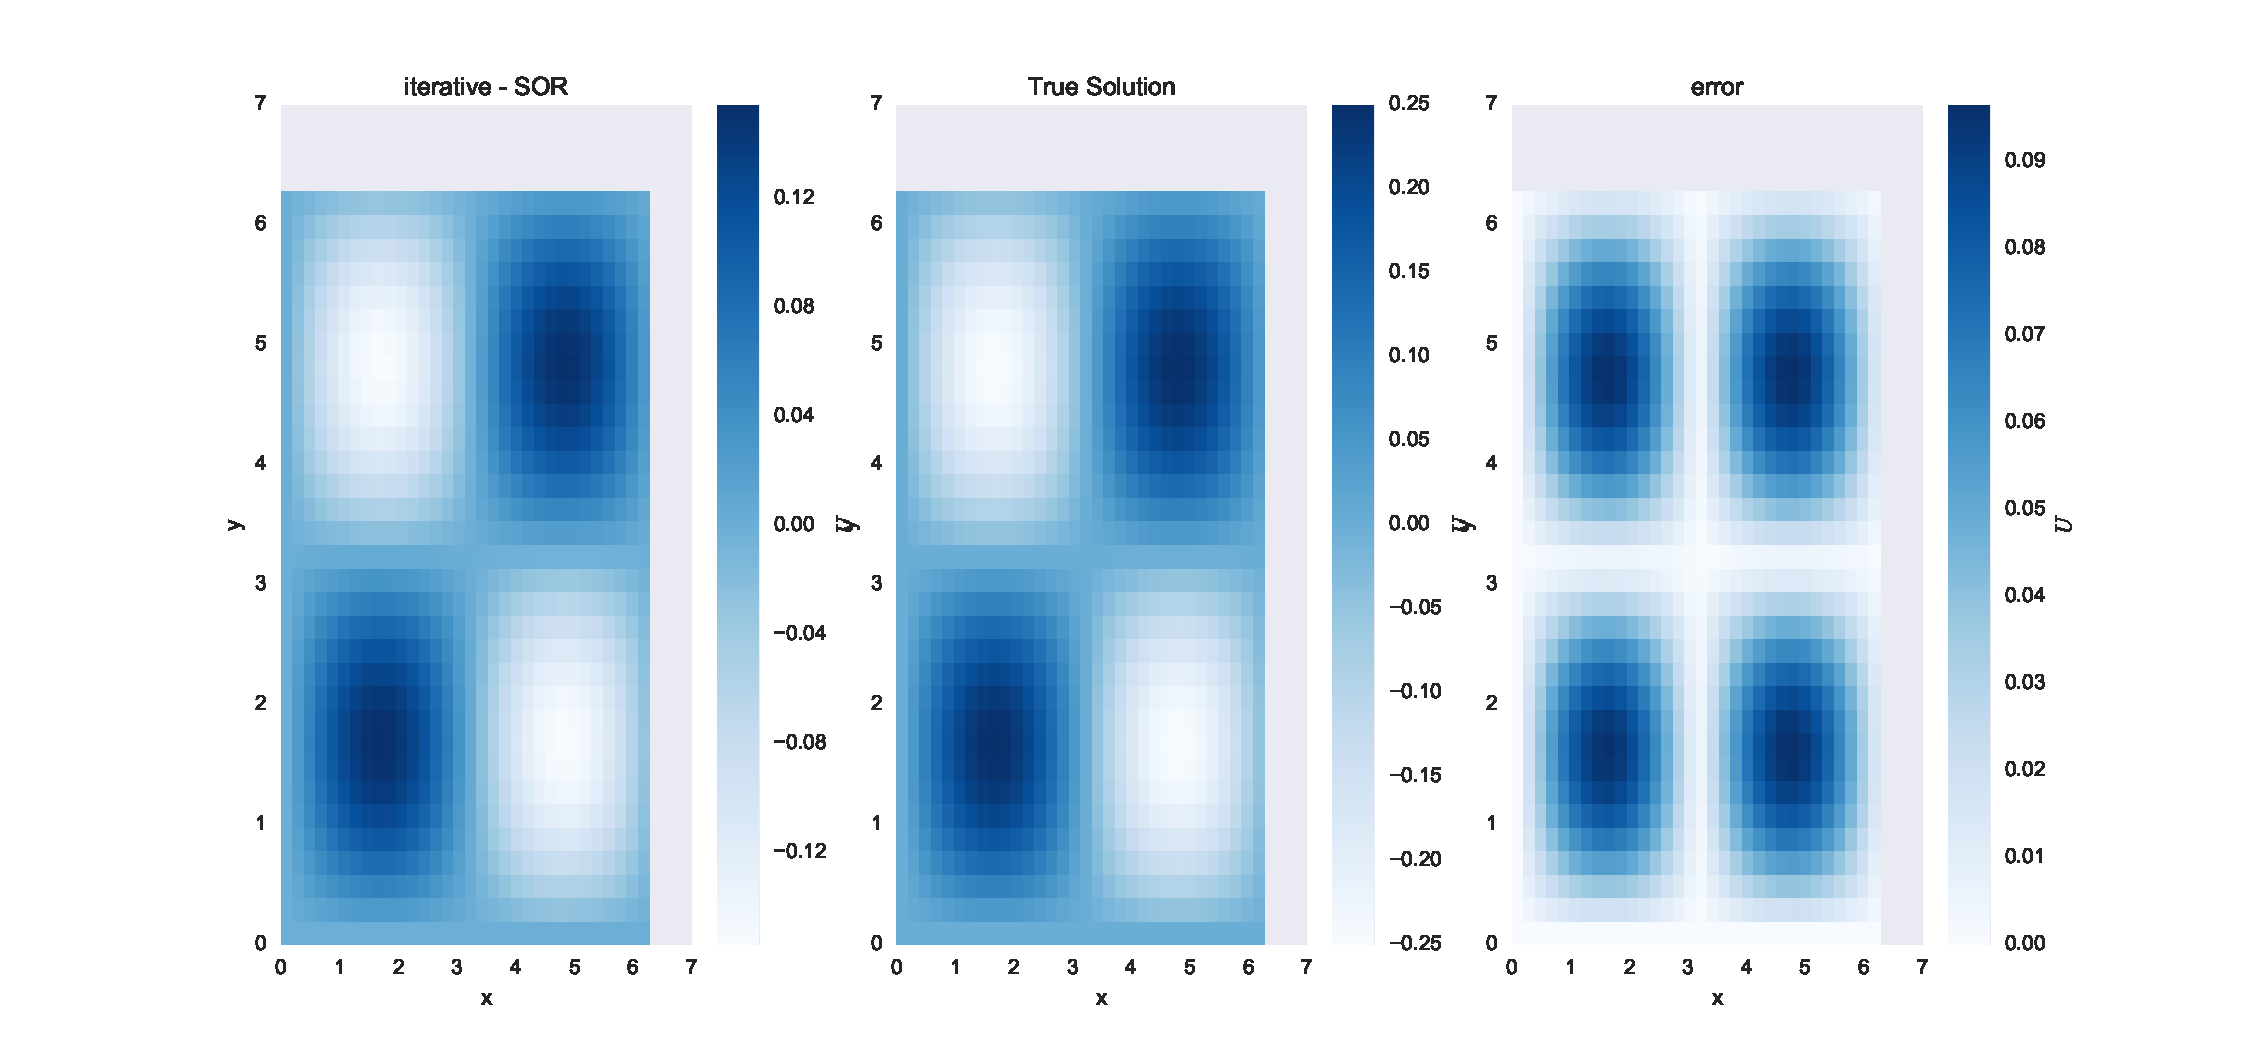
\includegraphics[scale=.5]{../plots/sor_sol_2d.pdf} \\
                \caption{(b)}
            \end{figure}
            
            \begin{figure}[!h]
                \centering
                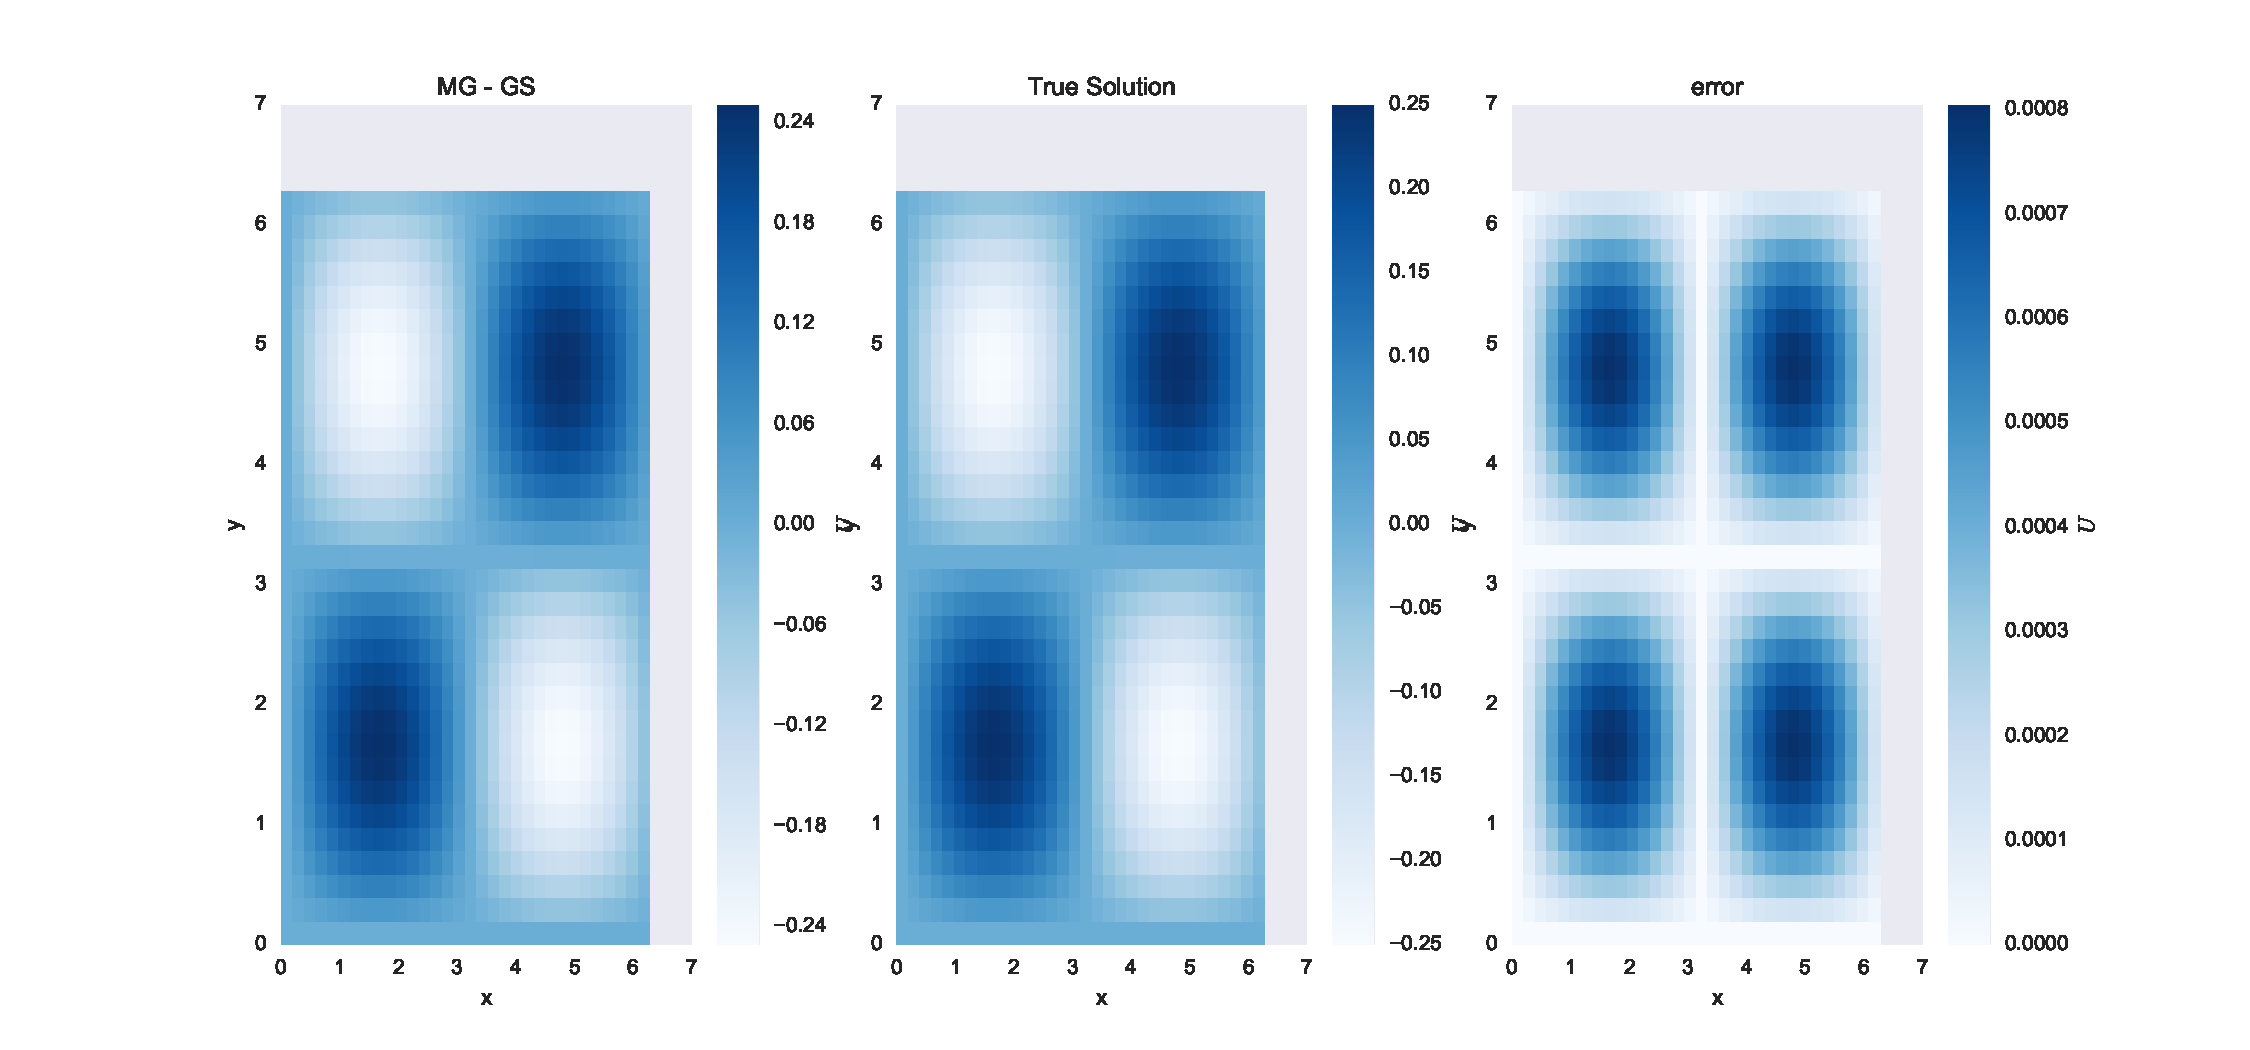
\includegraphics[scale=.5]{../plots/v_sol_2d.pdf} \\ 
                \caption{(c)}
            \end{figure}
            
            \begin{figure}[!h]
                \centering
                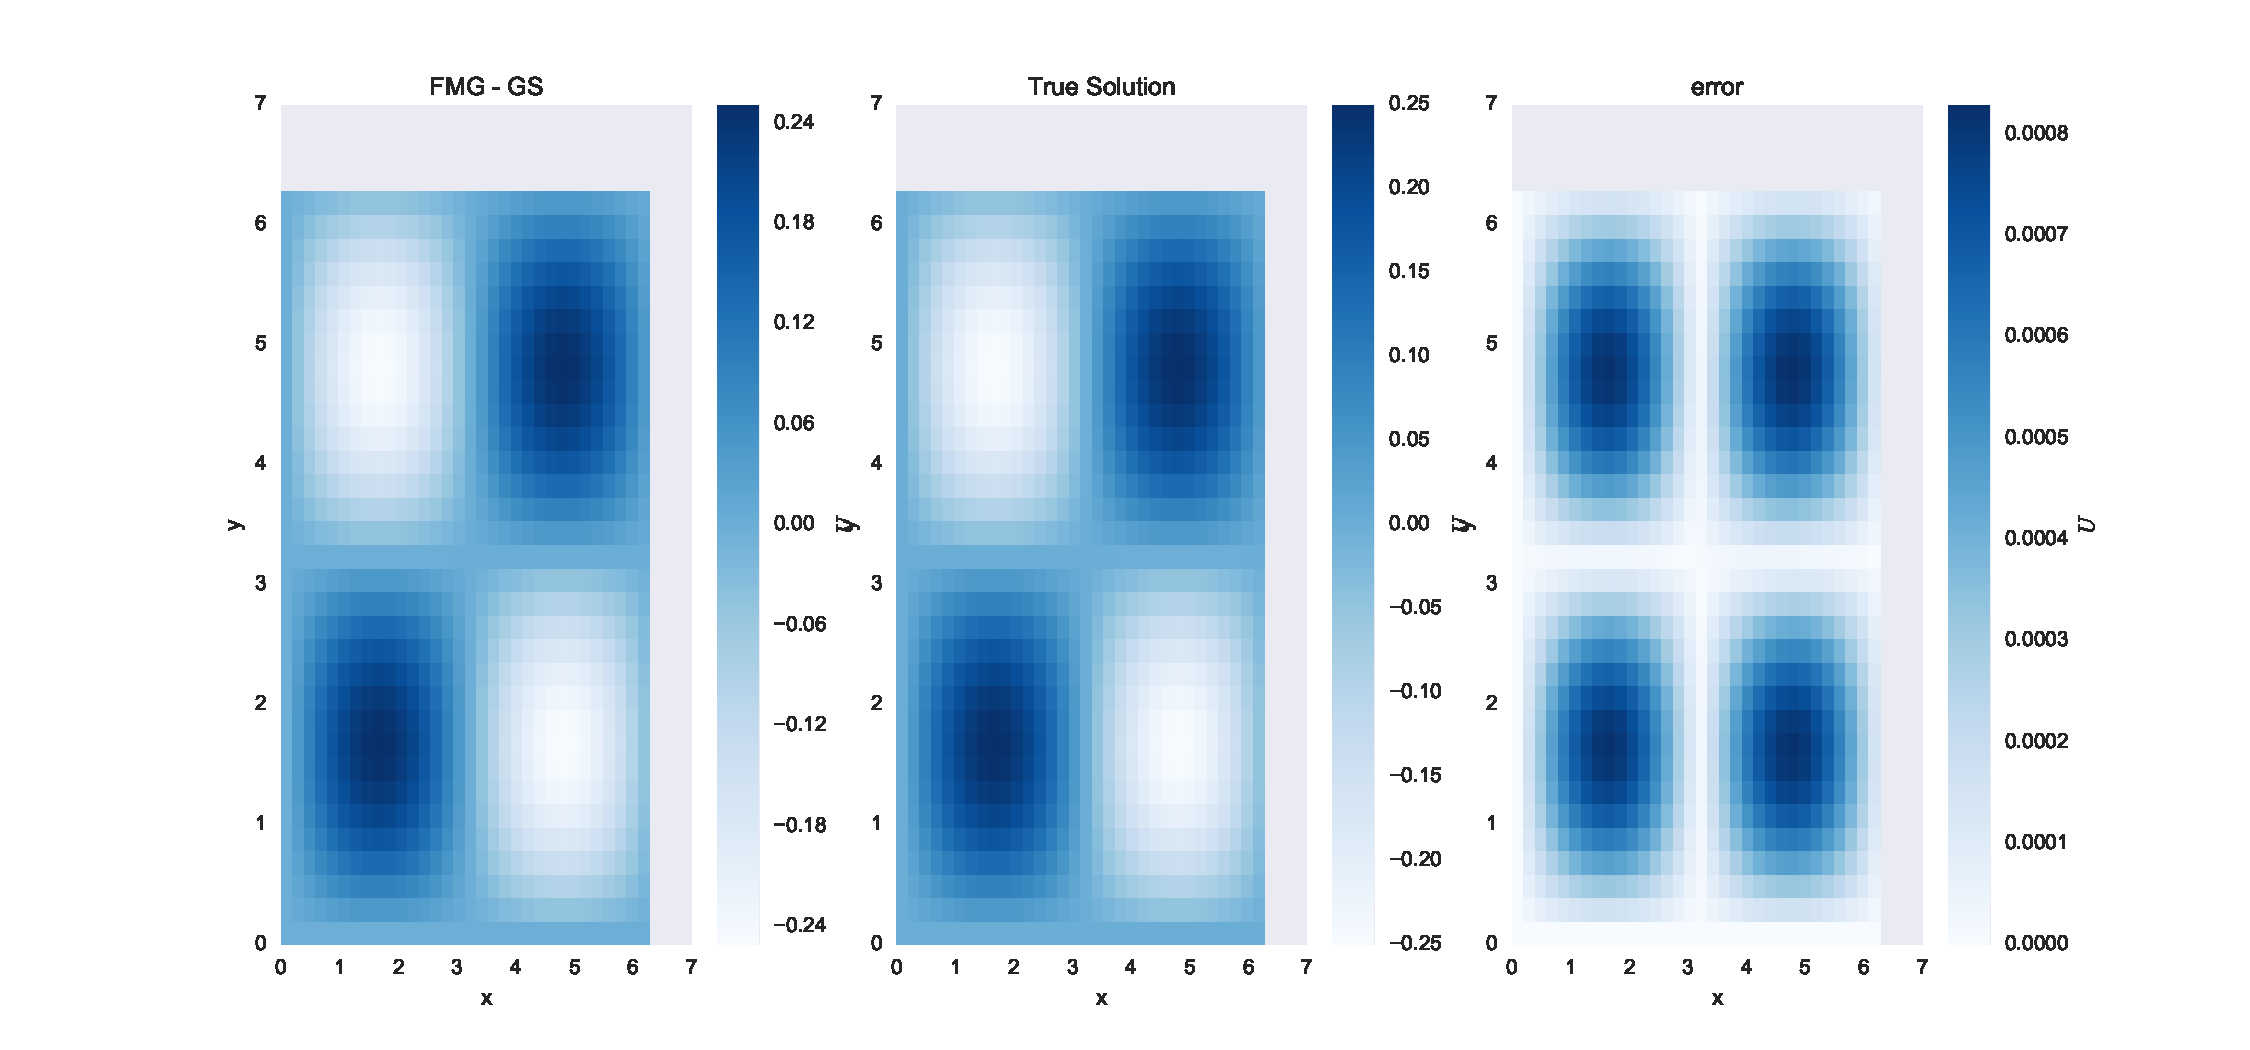
\includegraphics[scale=.5]{../plots/fmg_sol_2d.pdf} 
                \caption{(d)}
            \end{figure}
            
            \begin{figure}[!h]
                \centering
                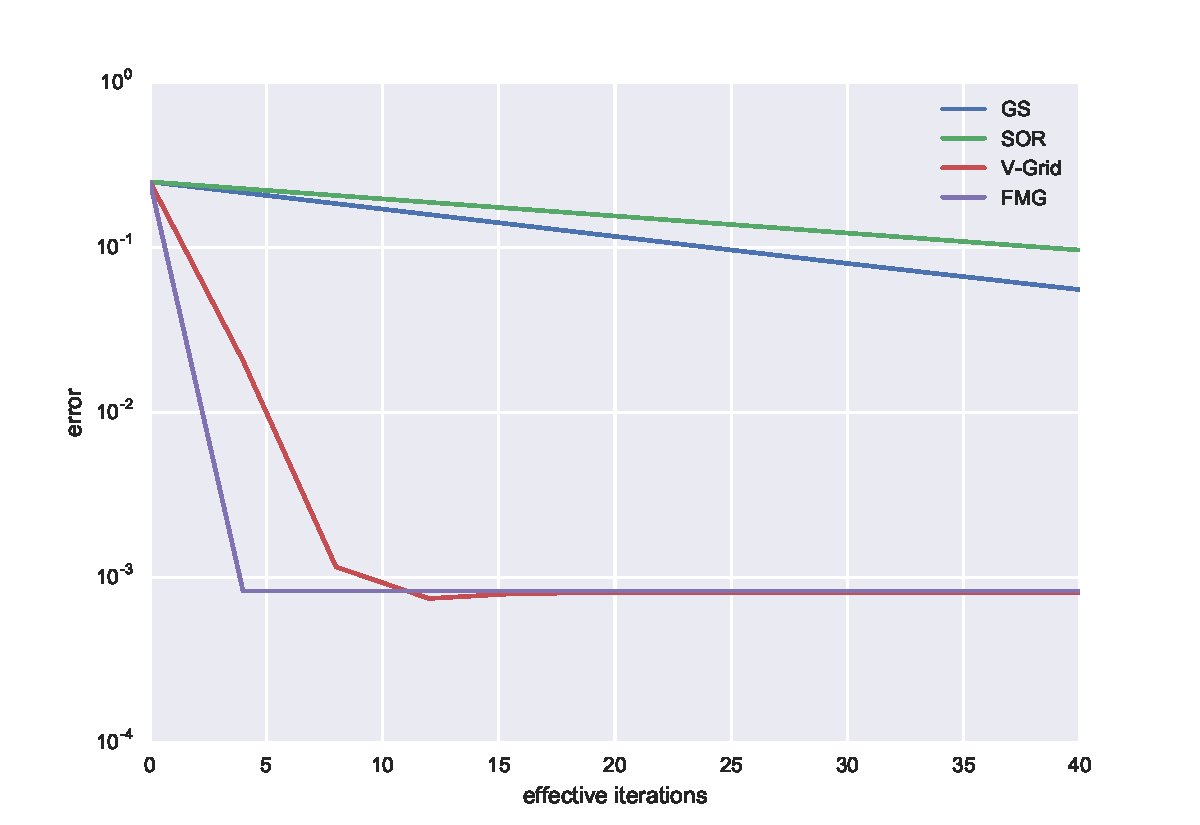
\includegraphics[scale=.75]{../plots/error_2d.pdf}
                \caption{Comparing error as a function of effective iteration in 2D}
            \end{figure}  

        \paragraph*{}

\newpage
\section{Error Analysis}

    \paragraph*{} The error analysis of multigrid methods falls back on the analysis of iterative methods. The multigrid methods converge with fewer sweeps than the iterative solver could on it's own. What's interesting about these methods is that the Full Multi Grid Cycle method converges as the descritization gets finer, independent of the number of sweeps! This is vastly different from the iterative methods alone, and even from the V-Cycle method. 
        \begin{figure}[h]
            \centering
            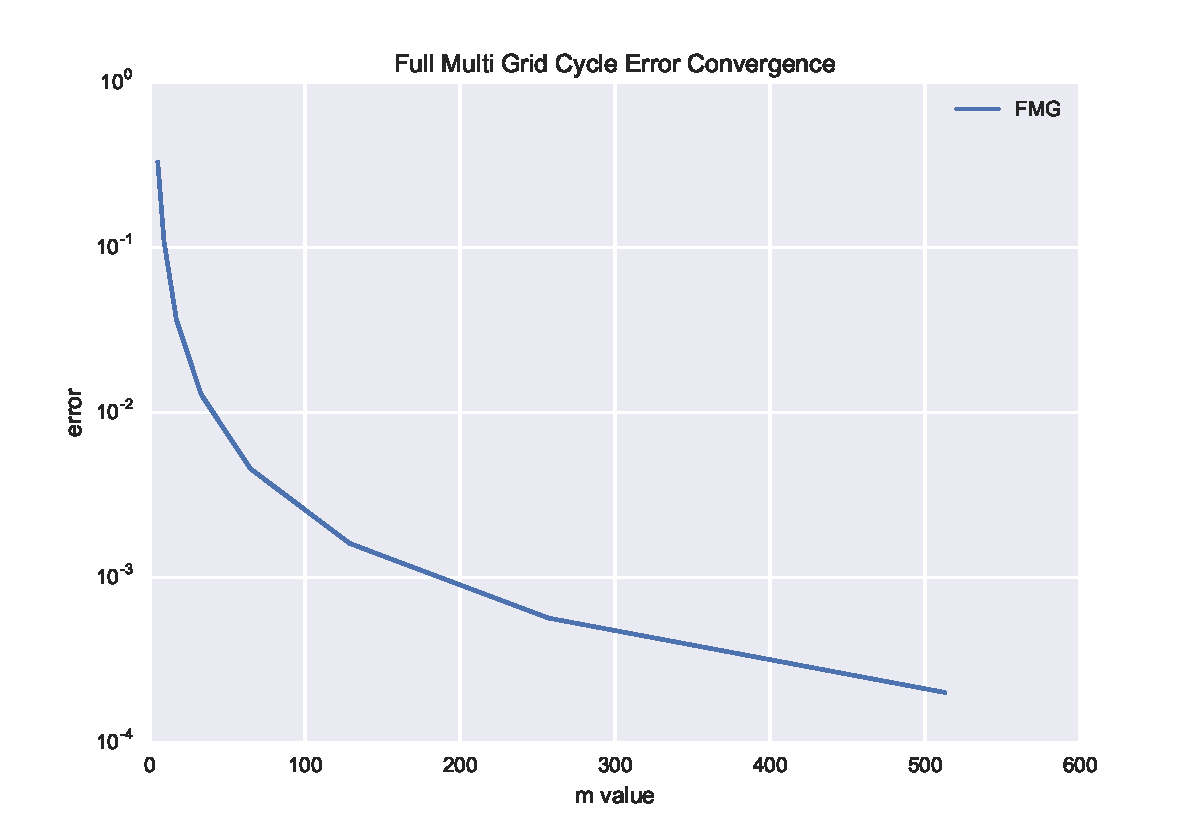
\includegraphics[scale=.4]{../plots/fmg_error.pdf}
            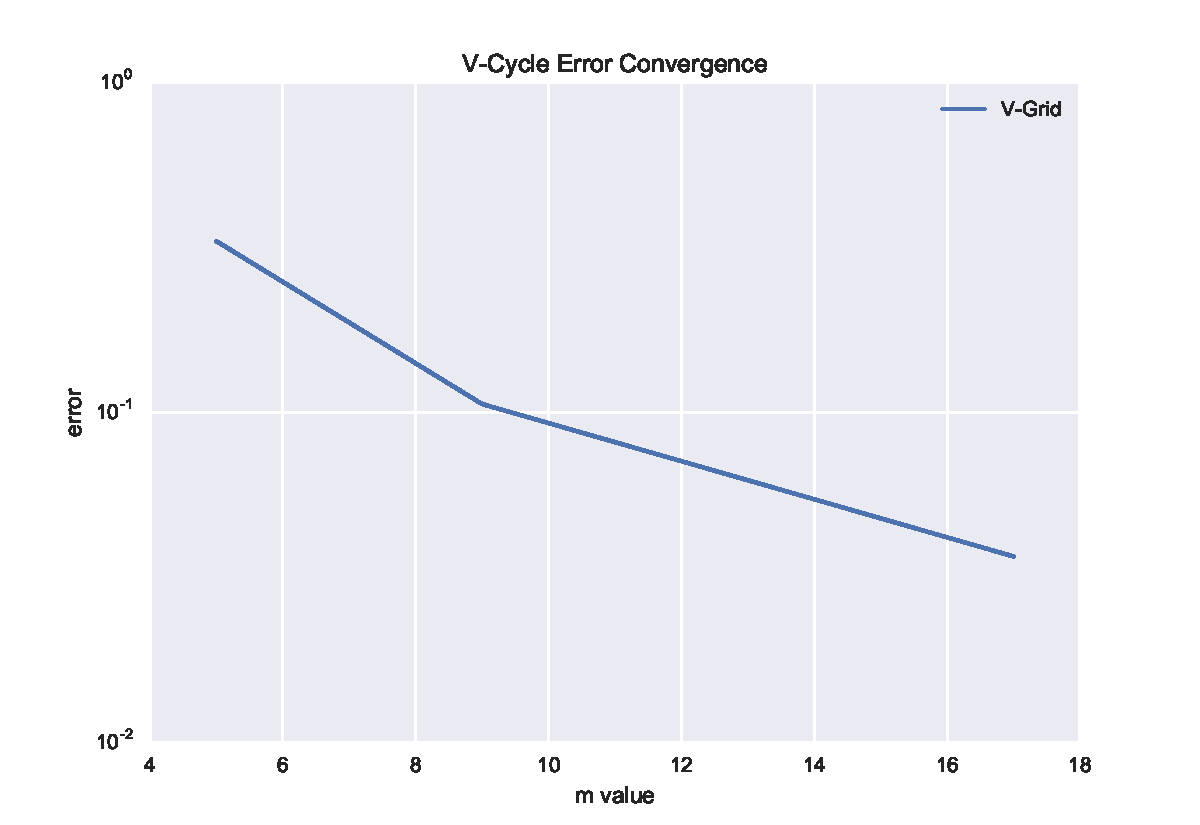
\includegraphics[scale=.4]{../plots/v_error.pdf}
        \end{figure}    
    The FMG method, plotted below on the left, converges as the descritization number $m$ goes up. At each $m$ value the \lstinline{fmg()} was called the same number of times. The V-Cycle method, whose error is below on the right, was run a little differently. \lstinline{v_sched()} was called $m$ times at each discritization $m$. This is more similar to the iterative smoothers on their own, which propogate information from the boundaries inward and therefore need more sweeps when there are more discrete points in the domain. 

\newpage
\section{Conclusion}
    
    \paragraph*{} Our implemation of multigrid methods leave somethings for future work. Most notably is treatment of non-zero boundary conditions. We found that while the linear system gets only marginally more complicated on paper, non-zero boundary conditions made the methods far more complicated. Additionally allowing the discretization to have $\Delta x$ different from $\Delta y$, would make a more robust method.

\section{Sources}  


\end{document}